\documentclass[14pt,aspectratio=169]{beamer}

\usepackage[english, spanish]{babel}
% \usepackage[T1]{fontenc}
% \usepackage[utf8]{inputenc}
\usepackage{minted}
\usepackage[nodayofweek,level]{datetime}
\usepackage{graphicx}
\usepackage{xcolor}
% \usepackage{simplebnf}
% \usepackage{multicol}
% \setlength{\columnsep}{0.2cm}

% %% Definiciones de comandos
\newcommand{\mydate}{\formatdate{29}{02}{2024}}
\graphicspath{ {images/} }
%%%%%%%%%%%%%%%%%%%%%%%%%%%%%%%%%%%%%%%%%%%%%%%%%%%%%%%%%%%%%%%%%%%%%%%%
%% Tema y estilo de la presentación
\usetheme{Madrid}
\author[Miguel E. Ruiz]{Miguel E. Ruiz}
\title[\texttt{Madrid |> Elixir}]{Cómo conocí a la metaprogramación\\ (y sobreviví a ello)}
\date{\mydate}

%%%%%%%%%%%%%%%%%%%%%%%%%%%%%%%%%%%%%%%%%%%%%%%%%%%%%%%%%%%%%%%%%%%%%%%%
%% Empieza el documento

\begin{document}

\begin{frame}
  \titlepage
\end{frame}

\begin{frame}{Contenidos}
  \tableofcontents[hideallsubsections]
\end{frame}

\section{Introducción}
\begin{frame}{\texttt{IO.puts("Hello, World!")}}
  \begin{columns}
    \begin{column}{0.5\textwidth}
      \centering
      
\includegraphics[width=0.8\textwidth]{me-formal.jpg}
    \end{column}

    \begin{column}{0.5\textwidth}
      \begin{itemize}
        \item \texttt{Miguel [Emilio]}
        \item Ingenierio Informático
        \item Intereses: Programación funcional y concurrente
        \item Erlang y Elixir
      \end{itemize}
    \end{column}
  \end{columns}
\end{frame}

\begin{frame}{La metaprogramación y yo}
  \begin{itemize}
    \item Al acabar el Grado (2018), interés en Elixir
    \begin{itemize}
      \item Ejercicios en Codewars
      \item Proyecto Pokedex
    \end{itemize}
    \item Interés en el libro \textit{Metaprogramming Elixir}
    \item Sin embargo\dots
    \begin{itemize}
      \item Falta de tiempo (y de motivación)
    \end{itemize}
    \item Arranca el máster (2021) y\dots
    \begin{itemize}
      \item recupero el interés en la metaprogramación
      \item posibilidad de hacer el TFM sobre ello
    \end{itemize}
  \end{itemize}
\end{frame}

\begin{frame}{Finalizadas las presentaciones\dots}
  
\includegraphics[width=0.8\textwidth]{calvin-hobbes.jpg}
\end{frame}

\section{Metaprogramación}
\begin{frame}{Metaprogramación}
  \begin{center}
    \Huge ¿KLK?
    \end{center}
\end{frame}

\begin{frame}{Metaprogramación}{Definicion(es)}
  \onslide<+->{\begin{block}{Elixir School}
    \textit{Metaprogramming is the process of using code to write code.}
  \end{block}}
  \onslide<+->{\begin{block}{Rust Web Programming}
    \textit{Metaprogramming can generally be described as a way in which the program
    can manipulate itself based on certain instructions.}
  \end{block}}
  \onslide<+->{\begin{block}{ChatGPT}
    \textit{Metaprogramming is a programming technique where a program can manipulate
    its own structure or behavior at runtime.}
  \end{block}}
\end{frame}

\begin{frame}{Metaprogramación}{Técnicas}
  \begin{itemize}
    \item Metaclases (Ruby, Python)
    \item Macros (Scala, Rust)
    \item Templates (C, C++)
  \end{itemize}
\end{frame}

\begin{frame}{Metaprogramación en Elixir}{Mi definición}
  \begin{itemize}
    \item Metaprogramación: mecanismo para generar programas a partir de
    otros programas (en tiempo de \underline{compilación}).
    \item Elixir tiene la capacidad de tratar los programas como un tipo de dato
    y modificarlos o transformarlos.
    \item Ejemplos de uso:
      \begin{itemize}
        \item Extensión del lenguaje a través de DSL.
        \item Creación de nuevas librerías como \textit{Phoenix} y \textit{Ecto}.
      \end{itemize}
  \end{itemize}
\end{frame}

\begin{frame}{Metaprogramación en Elixir}{¿Cómo?}
  \begin{itemize}
    \item A través de \underline{macros}, las cuales permiten \textbf{extender}
    el lenguaje
  \end{itemize}
  \begin{block}{¿Cuántas palabras reservadas hay en Elixir?}
    \begin{itemize}
      \item 8
      \item 15
      \item 37
      \item ninguna
    \end{itemize}
  \end{block}
\end{frame}

\begin{frame}{Metaprogramación en Elixir}{¿Cómo?}
  \begin{itemize}
    \item A través de \underline{macros}, las cuales permiten \textbf{expandir}
    el lenguaje
  \end{itemize}
  \begin{block}{¿Cuántas palabras reservadas hay en Elixir?}
    \begin{itemize}
      \item 8
      \item \textcolor{red}{15}
      \item 37
      \item ninguna
    \end{itemize}
    \mintinline{elixir}{true, false, nil, when, and, or, not, in}
    \mintinline{elixir}|fn, do, end, catch, rescue, after, else|
  \end{block}
\end{frame}

\begin{frame}{Metaprogramación en Elixir}{Proceso de compilación}
  \centering
  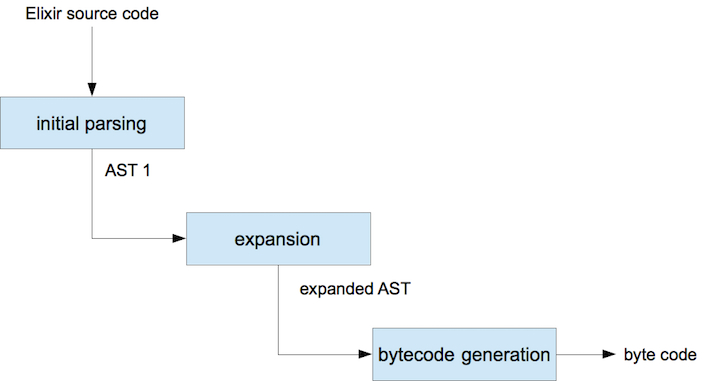
\includegraphics[width=0.6\textwidth]{compilation_process.png}
\end{frame}

\begin{frame}{Metaprogramación en Elixir}
  \begin{itemize}
    \item Con el operador \mintinline{elixir}|defmacro| podremos definir
    nuestras macros, respetando las reglas\footnotemark:
    \begin{itemize}
      \item Don't Write macros (WTF)
      \item Use Macros Gratuitously
    \end{itemize}
  \end{itemize}
  \footnotetext[1]{Metaprogramming Elixir: Macro Rules}
\end{frame}

\begin{frame}[fragile]{Metaprogramación en Elixir}{Ejemplos}
  \begin{columns}
    \begin{column}{0.5\textwidth}
      \scriptsize \begin{minted}{elixir}
        defmodule Sample.Weather do
          use Ecto.Schema
          schema "weather" do
            field :city
            field :temp_lo, :integer
            field :temp_hi, :integer
            field :prcp,    :float, default: 0.0
          end
        end
      \end{minted}
    \end{column}
    \begin{column}{0.5\textwidth}
      \scriptsize \begin{minted}{elixir}
        defmodule MyAppWeb.Router do
          use MyAppWeb, :router

          scope "/", MyAppWeb do
            pipe_through :browser

            get "/", PageController, :index
            get "/about", PageController, :about
          end
        end
      \end{minted}
    \end{column}
  \end{columns}
\end{frame}

\begin{frame}{AST (de Elixir)}
  \begin{itemize}
    \item Abstract Syntax Tree
    \item La estructura interna del código Elixir
    \item Se representa mediante una tupla de 3 elementos:
    \begin{itemize}
      \item Un átomo que representa la función invocada u otra tupla\\
      que representa un nodo interno del árbol.
      \item Una lista de términos de metadatos de la función invocada.
      \item Una lista de argumentos de la función del primer argumento.
    \end{itemize}
  \end{itemize}
\end{frame}

\begin{frame}[fragile]{AST de Elixir}
  Para obtener el AST de una expresión de Elixir, se utiliza la función
  \texttt{quote/2}:
  \footnotesize  \begin{minted}{elixir}
    iex> quote do: sum(1, 2, 3)
    {:sum, [], [1, 2, 3]}
  \end{minted}
  \normalsize Si se requiere introducir valores dentro de un AST, se dispone de la función
  \texttt{unquote/1}:
  \footnotesize \begin{minted}{elixir}
    iex> a = 3
    iex> quote do: sum(1, 2, a)
    {:sum, [], [1, 2, {:a, [], Elixir}]}
    iex> quote do: sum(1, 2, unquote(a))
    {:sum, [], [1, 2, 3]}
  \end{minted}
\end{frame}

\begin{frame}{Cosas para hablar}
  \begin{itemize}
    \item Hooks using y before\_compile
    \item Formas especiales \_\_MODULE\_\_ y \_\_ENV\_\_ y \_\_CALLER\_\_
  \end{itemize}

\end{frame}

\begin{frame}[fragile]{Ejemplos básicos}
  \begin{minted}{elixir}
    defmodule ControlFlow do
      defmacro unless(expression, do: block) do
        quote do
          if !unquote(expression), do: unquote(block)
        end
      end
    end
  \end{minted}
\end{frame}

\begin{frame}[fragile]{DEMO}{Un DSL para definir mascotas}
  \begin{columns}
    \begin{column}{0.5\textwidth}
      \scriptsize\begin{minted}{elixir}
        defmodule Example do
          use Pets

          pet "Bucky" do
            species :dog
            hobbies ["sniffing", "eating birds"]
          end
          defpet "Gardfield" do
            species :cat
            hobbies ["eating lasagna", "hating mondays"]
          end
        end
      \end{minted}
    \end{column}
    \begin{column}{0.5\textwidth}
      \scriptsize\begin{minted}{elixir}
        iex> Bucky.greet
        "Hello my name is Bucky and I'm a dog"
        iex> Gardfield.hobbies
        "Gardfield's hobbies are eating
        lasgna and hating mondays"
      \end{minted}
    \end{column}
  \end{columns}
\end{frame}

\begin{frame}{Antipatrones}

\end{frame}

\section{Mi TFM: \texttt{LogicElixir}}
\begin{frame}{\texttt{LogicElixir}}
  \begin{itemize}
    \item cosas a traer de la presentación del TFM
  \end{itemize}
\end{frame}

\begin{frame}{Bibliografía}
\end{frame}
\end{document}